\section{Durchführung}
\label{sec:Durchführung}
In Abbildung \ref{fig:Aufbau} ist der generelle Aufbau des Versuchs dargestellt.
Als Lichtquelle wird ein He-Ne-Laser benutzt, der monochromatisches, unpolarisiertes Licht bei einer Wellenlänge von $\qty{633}{\nano\meter}$ erzeugt.
Der Laser ist dabei anders als in der Abbildung fest. Dafür ist vor den Laser ein Polarisationsfilter
aufgestellt. Dabei ist das Licht senkrecht zur Einfallsebene polarisiert, wenn der Filter auf 0° eingestellt ist und parallel, wenn er 
auf 90° steht. Die zentrale Messapparatur ist ein sogenanntes Goniometer, was in Abbildung \ref{fig:Gonio} abgebildet ist.
Es besteht praktisch aus 3 unabhängigen Achsen. Die erste Achse, die mit der untersten Winkelskala gedreht werden kann, bewegt die gesamte Apparatur.
Die zweite Achse wird die über die Winkelskala darüber eingestellt und stellt den Spiegel relativ zur gesamt Apparatur ein.
Die dritte Achse ist ein Detektorarm, der unabhängig vom Rest eingestellt werden kann. Der Spiegel auf dem Goniometer kann sowohl in der Höhe als auch in 
der Ausrichtung über Klemmschrauben verstellt werden. Der Detektor ist an ein Amperemeter angeschlossen, um die gemessene Intensität zu quantifizieren 

\begin{figure}[H]
    \centering
    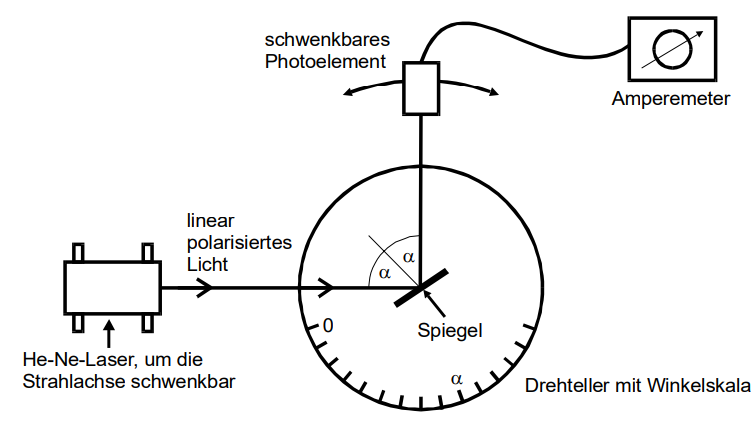
\includegraphics[scale=1]{content/Aufbau.png}
    \caption{Versuchsaufbau zur Bestimmung der Winkelabhängigkeit der Intensität des reflektierten Lichts \cite{sample}.}
    \label{fig:Aufbau}
\end{figure}
\begin{figure}[H]
    \centering
    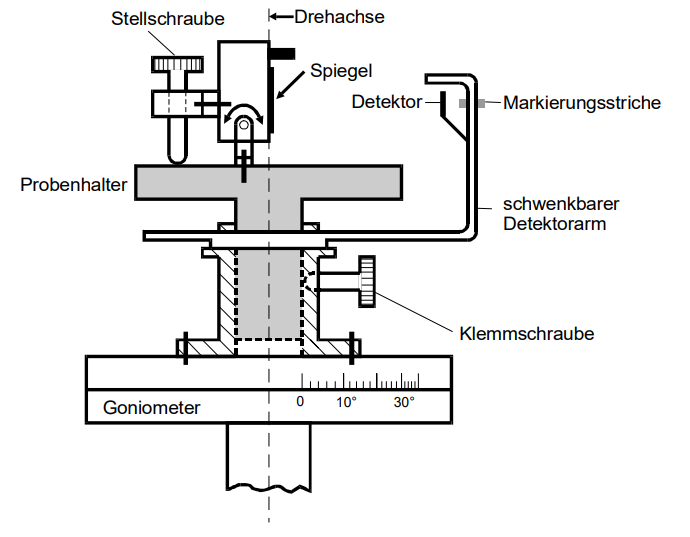
\includegraphics[scale=1]{content/Goniometer.png}
    \caption{Schematische Darstellung des Goniometers \cite{sample}.}
    \label{fig:Gonio}
\end{figure}

\noindent Um nun die winkelabhängige Intensitätsverteilung zu bestimmen muss die Messapparatur zunächst richtig kalibriert werden.
Dafür werden zunächst die Apparaturachse und die Spiegelachse parallel auf 0° gestellt. Beide Achsen werden dann zusammen so ausgerichtet, dass der Laserstrahl möglichst
parallel auf den Polarisationsfilter zurückgeworfen wird. Der Spiegel wird in der Höhe so eingestellt, dass der Laserstrahl möglichst zentral auftrifft. Die Orientierung wird so gewählt, dass der Laserstrahl den Detektor zentral trifft.
Nun ist die Apparatur bereit zur Messung. Der Polarisationsfilter wird in einer Messung auf 0° und in der anderen auf 90° gestellt.
Für beide Messreihen wird jetzt in 2° Schritten von 6° bis 90° gemessen. Dabei wird die Apparatur Winkelscheibe festgehalten und
die Spiegelachse gemäß Skala um jeweils 2° gegenüber der Apparatur Achse verschoben. Danach werden beide Achsen festgehalten und der 
Detektor wird so bewegt, dass der Laserstrahl exakt den Detektor trifft. Es kommt hier auf höchste Präzision an. Wir haben uns am Amperemeter orientiert. Das heißt wir haben so lange gedreht
bis der Detektor eine maximale Intensität verzeichnet hat. Dann sind wir davon ausgegangen, dass der Detektor den Laserstrahl optimal detektiert.
Bei sehr niedrigen Winkeln, kleiner 6°, und großen Winkeln, in der Nähe von 90°, ist entweder der Detektor im Weg des einfallenden Laserstrahls oder der Laserstrahl
hat den Spiegel nicht mehr vollständig getroffen. Neben der Messung des reflektierten Strahls, soll auch für beide Polarisationsrichtungen einmal die einfallende Intensität gemessen werden.
Dafür wird der Spiegel ausgebaut und der Detektor direkt in den Laserstrahl gestellt. Im Zustand ohne Spiegel soll außerdem noch die Polarisationsrichtung 
mit der geringsten durchkommenden Intensität gemessen werden und der Dunkelstrom. Dafür soll der Detektor möglichst weit weg vom Laser orientiert werden. Die gemessene Intensität 
entspricht dem Dunkelstrom.